\chapter{Shell的基本用法}
\label{cp:shellusage}

\section{Shell简介}

\subsection{概述}

\textbf{Shell是计算机中一种重要的命令行解释器},其主要功能是\textit{接收用户输入的命令,并将其传递给操作系统内核进行处理}。实际上,它\textit{提供了与操作系统交互的接口},使得用户能够textit{通过命令行完成各种任务},如文件管理、系统配置和进程控制。Shell的发展历史悠久,其在Unix和类Unix发行版中都扮演着关键角色。\\

从\textbf{工作原理上看},Shell通过\textit{解析用户输入的命令,将其转化为内核能够理解的系统调用,进而控制系统资源完成任务}。其基本操作模式是\textbf{交互式}的:用户输入一条命令后,Shell会对其进行解析,并决定如何执行。若\textit{该命令是系统内置的Shell命令,则直接调用Shell的内置函数处理;若是外部命令,则通过查找系统中的可执行文件,调用相应的程序。}用户与Shell的这种\textbf{互动一般通过命令行界面(CLI)进行,每次操作都包括输入、执行和输出的完整流程。}\\

更进一步地,\textbf{Shell还支持脚本编写功能},是更高级的定制和自动化,用户可以将一系列命令\textit{写入脚本文件,Shell会按顺序逐条执行。}这是Shell作为系统管理和自动化任务中最重要工具的原因,也正因此,用户可以轻松实现批量文件处理、系统监控以及软件安装等复杂任务。

\subsection{Shell的类型}

在实际应用中,\textbf{Shell有多种类型},其中最常见的\textit{包括 Bash (Bourne Again Shell)、Zsh (Z Shell) 和 Fish (Friendly Interactive Shell) 等。}\\

\textbf{Bash 是目前最广泛使用的 Shell 类型},作为 GNU 项目的一部分,不仅兼容早期的 Bourne Shell,还增加了许多新功能,如命令行自动补全和历史记录机制。\textbf{Zsh 则是一种功能更强大且高度可定制化的 Shell},继承了 Bash 的所有特性,同时引入了更为先进的自动补全、插件支持以及更灵活的脚本编写能力。\textbf{Fish 则以简单易用著称},设计目标是为用户提供更直观的命令行体验,尤其适合新手。\\

\textbf{这些不同的 Shell 工具,实际上都在不同的类 Unix 发行版中被使用},不同的 Linux 发行版对 Shell 的支持也存在差异。\textit{大多数现代 Linux 发行版,如 Ubuntu、Debian、CentOS 等,都默认使用 Bash 作为其标准的命令解释器。}然而,有些发行版,\textit{如 Arch Linux 和 macOS,在提供 Bash 的同时,也预装了 Zsh 或其他类型的 Shell}。发行版选择 Shell 的标准通常基于其稳定性、功能性和用户的使用习惯。由于开源系统的性质,用户可以根据个人偏好,在系统中安装并切换不同的 Shell。

\section{Shell基本指令}

\subsection{基本指令概述}

下表中的Shell指令,是我在大一时学习\textit{Missing Semester}课程时总结的,也包含了我在Linux服务器运维的一些经验。具体见表\ref{tab:shellcommands}。\footnote{由于当时接触MIT - Missing Semester我更偏向于使用英文,所以这里的表格也是根据当时使用英文编写的完善。}

\begin{longtable}{|l|p{5cm}|p{8cm}|}
\hline
\textbf{Name} & \textbf{Usage} & \textbf{Details} \\
\hline
\endfirsthead
\hline
\textbf{Name} & \textbf{Usage} & \textbf{Details} \\
\hline
\endhead
\hline
\endfoot

\texttt{ls} & \texttt{ls -l}: long format & \textit{List directory contents} \\
\hline
\texttt{man} & \textit{Shows you its manual page} & Displays the manual page of a command for detailed help \\
\hline
\texttt{cp} & \textit{Copy files or directories} & \textbf{cp} is used to copy one or more files to another location. It can also copy directories when used with \texttt{-r}. \\
\hline
\texttt{mkdir} & \textit{Make directory} & Creates a new directory with the specified name \\
\hline
\texttt{rmdir} & \textit{Can only remove empty directory} & Deletes a directory, but only if it is empty. For non-empty directories, \texttt{rm -r} is required. \\
\hline
\texttt{rm} & \texttt{rm -r}: remove directories and their contents recursively & \textit{Removes files or directories}. Be careful when using \texttt{rm -r} as it will delete the directory and all of its contents recursively. \\
\hline
\texttt{su} & \texttt{sudo su}: switch to root & Switches user (usually to root). \textbf{su} allows the user to assume another user's identity, typically root. \\
\hline
\texttt{sudo} & \textit{Do something as superuser (“root”)} & Allows a permitted user to execute a command as the superuser or another user. Commonly used for administrative tasks. \\
\hline
\texttt{tee} & \texttt{-a} = --append (not overwrite) & Reads from standard input and writes to both standard output and files. For example, \texttt{echo 3 | sudo tee brightness} modifies a file with the new input. \\
\hline
\texttt{cat} & \textit{Concatenate and display file contents} & Concatenates files and displays their content. Often used for reading files. \\
\hline
\texttt{tail} & \texttt{tail -n 10}: display the last 10 lines & Displays the last part of a file, often useful for viewing logs. The \texttt{-f} option can be used to follow updates in real-time. \\
\hline

\caption{常用Shell指令}
\label{tab:shellcommands}

\end{longtable}

特别的,\texttt{ls}指令有现代的衍生版本,如\texttt{eza},可以提供更多的功能和更好的用户体验。

\subsection{实例演示}
\label{cp:shellcommands-demo}

\textbf{下面是一些常见的Shell指令的实例演示},以更好地理解其用法。所有演示均在我的\textit{Ubuntu 22.04.04 LTS Azure SG Server}上完成。\\

第一组示例,我们将演示\textit{基本的文件操作}。请见代码\ref{listing:shellcommands1}。

\begin{longlisting}
    \begin{minted}{bash}
# 确认当前目录
pwd
## 输出:/home/JStar0Y

# 列出当前目录下的所有文件
ls
# 如果想要更加详细的信息,可以使用 -l 选项;至于 -a 选项,可以显示隐藏文件
ls -al
## drwxr-x--- 5 JStar0Y JStar0Y     4096 Sep 13 03:27 .
## drwxr-xr-x 3 root    root        4096 Jul  8 17:18 ..
## -rw-r--r-- 1 JStar0Y JStar0Y      807 Jan  6  2022 .profile
## drwx------ 2 JStar0Y JStar0Y     4096 Jul  8 17:18 .ssh
## ... 其他文件省略 ..

# 创建一个新的目录
mkdir test

# 移动到新创建的目录
cd test

# 创建一个新的文件
touch test.txt

# 删除刚才创建的文件
rm test.txt
# 如果要删除非空文件夹,需要使用 -r 选项(recursively)

# 返回上一级目录
cd ..

# 删除刚才创建的目录(如果非空则无法使用 rmdir)
rmdir test
    \end{minted}
    \caption{Shell常用指令实例一:文件操作}
    \label{listing:shellcommands1}
\end{longlisting}

第二组演示,我们将展示\textit{如何使用\texttt{sudo}和\texttt{su}命令}。请见代码\ref{listing:shellcommands2}。

\begin{longlisting}
    \begin{minted}{bash}
# 查看当前用户
whoami
## 输出:JStar0Y

# 使用 sudo 切换到 root 用户
sudo su
# 此处我因为我修改过 sudoers 文件,所以不需要输入密码
# 更一般的操作系统,需要输入当前用户的密码(前提是当前用户拥有 sudo 权限)

# 查看当前用户
whoami
## 输出:root

# 退出 root 用户
exit

# 使用 su 切换到 root 用户
su
# 输入 root 用户的密码后,切换成功
# 一般的,su 后面可以跟用户名,用于切换到其他用户,密码也是对应的用户密码
    \end{minted}
    \caption{Shell常用指令实例二:\texttt{sudo}和\texttt{su}命令}
    \label{listing:shellcommands2}
\end{longlisting}

第三个示例,我们将展示\textit{如何使用\texttt{tee}、\texttt{tail}和\texttt{cat}命令}。请见代码\ref{listing:shellcommands3}。

\begin{longlisting}
    \begin{minted}{bash}
# 使用 tee 命令将输入写入文件
echo "Hello, World!" | sudo tee test.txt

# 使用 cat 命令查看文件内容
cat test.txt

# 使用 tee 命令追加内容
echo "Hello, World Again!" | sudo tee -a test.txt

# 使用 tail 命令查看文件末尾内容
tail test.txt
# 如果想要实时查看文件内容,可以使用 -f 选项
# 此处的 & 用于将进程放入后台,以便继续输入其他命令
tail -f test.txt &
# 此时,对文件修改
echo "Hello, World Again and Again!" | sudo tee -a test.txt
## 输出:Hello, World Again and Again!
## 因为后台有 tail 命令,所以会实时显示文件内容

# 结束 tail 命令
kill %1
    \end{minted}
    \caption{Shell常用指令实例三:\texttt{tee}和\texttt{cat}命令}
    \label{listing:shellcommands3}
\end{longlisting}

此处需要注意,\texttt{|}左右两侧的命令不可以互换。关于这点,我们在第\ref{cp:piperedirection}节中马上介绍。

\section{数据管道与重定向}

\label{cp:piperedirection}

\subsection{何谓数据管道与重定向}

\textbf{数据管道是 Shell 中的一种重要概念},它\textit{允许将一个命令的输出作为另一个命令的输入},从而实现多个命令之间的数据传递。数据管道的符号是 \texttt{|},它将两个命令连接在一起,使得第一个命令的输出成为第二个命令的输入。例如,\texttt{ls | grep .txt} 将列出当前目录下的所有文件,并将包含 \texttt{.txt} 的文件名过滤出来。\\

\textbf{而重定向是 Shell 中的另一种重要概念},\textit{允许将命令的输入和输出重定向到文件}。重定向的符号有 \texttt{<} 和 \texttt{>},分别表示输入重定向和输出重定向。例如,\texttt{ls > files.txt} 将列出当前目录下的所有文件,并将结果保存到 \texttt{files.txt} 文件中。

\subsection{管道与重定向操作概述}

类似的,该部分也是我在大一时学习\textit{Missing Semester}课程时总结的,是根据当时使用英文编写的完善。\\

Operations like \texttt{|}, \texttt{>}, and \texttt{<} are done \textit{by the shell}, not by the individual program:

\begin{enumerate}

    \item pipe: \texttt{|} \textbf{take the output} of the program to the \textit{left} and \textbf{make it the input} of the program to the \textit{right}.

    \item \texttt{<} indicates rewire the \textbf{input} for this program to be the \textbf{contents of the file \textit{(READ FILE)}}
    
        \texttt{>} means rewire the \textbf{output} of the preceding program \textbf{into this file \textit{(WRITE FILE)}}

        \texttt{>>} \textbf{is like} \texttt{>}, but \textbf{append to a file}.

\end{enumerate}

特别的,\texttt{|}两侧的权限是不同的,如果在左侧使用\texttt{sudo},右侧的命令不会继承\texttt{sudo}的权限。

\subsection{联用组合命令}

\textbf{Shell 中的管道和重定向操作可以联用其他工具},以实现更复杂的数据处理需求。例如,\texttt{ls | grep .txt > files.txt} 将列出当前目录下的所有文件,并将包含 \texttt{.txt} 的文件名保存到 \texttt{files.txt} 文件中。\\

\textbf{这种联用组合命令的方式,可以实现更多的功能},如文件搜索、数据过滤、日志分析等。根据具体需求,将多个命令组合在一起,就实现了更为复杂的数据处理任务。

\subsection{实例演示}

依然如\ref{cp:shellcommands-demo}节,我们将展示\textit{如何使用管道和重定向操作},并\textit{联用组合命令}。\\

第一组示例,我们将演示\textit{如何使用基本的管道操作}。请见代码\ref{listing:piperedirection1}。

\begin{longlisting}
    \begin{minted}{bash}
# 列出当前目录下的所有文件,并将包含 .txt 的文件名过滤出来
ls | grep .txt

# 写入./test/test.txt文件一些内容
echo "Hello, World!" > ./test/test.txt

# 追加内容
echo "Hello, World Again!" >> ./test/test.txt

# 查看文件内容
cat ./test/test.txt
## 输出:Hello, World!

# 查看文件内容,并将包含 World 的行过滤出来
cat ./test/test.txt | grep World
## 输出:Hello, World!
##      Hello, World Again!

# 然而,如果再使用 >,会覆盖原有文件内容
echo "Hello, World, Twice!" > ./test/test.txt
cat ./test/test.txt
## 输出:Hello, World, Twice!
## 这告诉我们,如果要追加内容,需要使用 >>

# 从文件中读取内容
cat < ./test/test.txt
# 其实,这个命令等价于 cat ./test/test.txt
# 但是这里使用了输入重定向的用法

# 从文件中读取内容,并将包含 World 的行过滤出来
cat < ./test/test.txt | grep World
## 输出:Hello, World, Twice!

# 从一个文件中读取内容,并将其写入另一个文件,并查看另一个文件内容
cat < ./test/test.txt > ./test/test2.txt && cat ./test/test2.txt
# 注意此处 && 的用法在部分Linux发行版中可能会有不同
    \end{minted}
    \caption{Shell管道和重定向操作实例一}
    \label{listing:piperedirection1}

\end{longlisting}

第二组示例,我们将展示\textit{如何使用联用组合命令},主要展示\texttt{grep, awk, sed}这几个工具。请见代码\ref{listing:piperedirection2}

\begin{longlisting}
    \begin{minted}{bash}
# 使用 grep 过滤文件内容
cat /etc/passwd | grep root
## 将输出系统中存储的所有包含 root 的行,即
## root:x:0:0:root:/root:/bin/bash

# 使用 awk 过滤文件内容
# awk options 'pattern {action}' file
cat /etc/passwd | awk -F: '{print $1}'
# 这里的 -F: 表示使用 : 作为分隔符
# $1 表示第一个字段,即用户名
## 将输出系统中存储的所有用户名

# 使用 sed 过滤文件内容
# sed [-hnV][-e<script>][-f<script文件>][文本文件]
cat /etc/passwd | sed -n '1,3p'
# 这里的 -n 表示只输出匹配的行
# 1,3p 表示输出第 1 行到第 3 行
## 将输出系统中存储的前三行内容,即
## root:x:0:0:root:/root:/bin/bash
## daemon:x:1:1:daemon:/usr/sbin:/usr/sbin/nologin
## bin:x:2:2:bin:/bin:/usr/sbin/nologin
    \end{minted}
    \caption{Shell管道和重定向操作实例二}
    \label{listing:piperedirection2}
\end{longlisting}

\section{基本的Shell脚本编写}

\subsection{Shell脚本概述}

\textbf{Shell脚本强大的工具},广泛应用于\textit{自动化任务和系统管理}。脚本语言拥有简洁和灵活的特性,用户能够快速编写脚本来完成复杂的任务。编写脚本的基础是\textit{掌握其基本语法结构、变量处理、条件判断与循环等操作},这些是实现功能的核心。

\subsection{Shell脚本基本语法}

\subsubsection{变量的定义}

Shell 脚本中,\textbf{变量的使用和运算非常重要}。变量无需预先声明,可以直接通过赋值来创建。例如,通过\texttt{my\_var=5}可以定义一个名为\texttt{my\_var}的变量,其值为\texttt{5}。\\

特别需要注意的是,\textbf{变量在Shell中默认为字符串形式},进行数值运算时,必须通过\texttt{expr}或 \texttt{\$(())} 等方式进行。例如,\texttt{result=\$((\$my\_var + 2))}才是正确的。\\

脚本中,还可以\textbf{通过命令替换,将命令的输出赋值给变量},例如\texttt{current\_date=\$(date)}会将当前日期赋值给\texttt{current\_date}变量,而其中的\texttt{\$(date)}是一个命令替换操作,会将\texttt{date}命令的输出作为变量的值。\\

\subsubsection{条件判断}

\textbf{条件判断是脚本控制流中不可或缺的一部分。}在 Shell 脚本中,\textit{if-else 语句用于实现逻辑判断。if 语句通过 \texttt{[]} 或 \texttt{test} 命令进行判断操作。}\\

特别地,\textbf{Shell 判断语法中的空格要求非常严格},[] 内的表达式必须用空格分隔。我们给出一个简单的例子,如代码\ref{listing:shellscript1}所示。

\begin{longlisting}
    \begin{minted}{bash}
# 定义一个变量
my_var=5

# 判断变量是否大于 2
if [ $my_var -gt 2 ]; then
    echo "my_var is greater than 2"
else
    echo "my_var is less than or equal to 2"
fi

## 或者使用 test 命令来进行判断
if test $my_var -gt 2; then
    echo "my_var is greater than 2"
else
    echo "my_var is less than or equal to 2"
fi
    \end{minted}
    \caption{Shell脚本基本语法示例一}
    \label{listing:shellscript1}
\end{longlisting}

\subsubsection{循环结构}

提供两种循环结构:\textit{for 循环和 while 循环}。for 循环用于遍历一个列表,while 循环则用于根据条件执行循环。具体的语法如代码\ref{listing:shellscript2}所示。

\begin{longlisting}
    \begin{minted}{bash}
# for 循环
for i in 1 2 3 4 5
do
    echo "Number: $i"
done

for file in /tmp/*; do
    echo "发现文件: $file"
done

# while 循环
count=0
while [ $count -lt 5 ]; do
    echo "Count: $count"
    count=$((count + 1))
done
    \end{minted}
    \caption{Shell脚本基本语法示例二}
    \label{listing:shellscript2}
\end{longlisting}

\subsection{实战:编写一个垃圾清理脚本}

首先建立基本的思路——\textit{脚本应该检查缓存目录是否存在,如果不存在则输出错误日志并退出。接着,使用 rm -rf 命令清空缓存目录,并将结果记录到日志文件中。通过将 date 命令与变量结合,我们能够在日志中记录清理操作的时间戳。}具体实现见代码\ref{listing:shellscript3}。

\begin{longlisting}
    \begin{minted}{bash}
#!/bin/bash

# 定义变量
CACHE_DIR="/var/cache"
LOG_FILE="/var/log/cache_cleanup.log"
TIMESTAMP=$(date "+%Y-%m-%d %H:%M:%S")

# 检查缓存目录是否存在
if [ ! -d "$CACHE_DIR" ]; then
    echo "$TIMESTAMP - 错误: 目录 $CACHE_DIR 不存在" >> $LOG_FILE
    exit 1
fi

# 清理缓存
echo "$TIMESTAMP - 开始清理 $CACHE_DIR" >> $LOG_FILE
rm -rf $CACHE_DIR/*

# 确认清理成功
if [ $? -eq 0 ]; then
    echo "$TIMESTAMP - 缓存清理完成" >> $LOG_FILE
else
    echo "$TIMESTAMP - 错误: 清理失败" >> $LOG_FILE
    exit 1
fi
    \end{minted}
    \caption{Shell脚本实战:垃圾清理脚本}
    \label{listing:shellscript3}
\end{longlisting}

将上述脚本保存在 \texttt{cleanup.sh} 文件中,然后通过 \texttt{chmod +x cleanup.sh} 命令添加执行权限。接着,运行 \texttt{./cleanup.sh} 命令,即可执行脚本。或者,不添加权限,我们直接使用 \texttt{bash cleanup.sh} 命令执行脚本。\\

直接运行我们会发现,\textit{权限不足},此时我们需要使用\texttt{sudo}命令来执行脚本。执行结果见图\ref{fig:shellscript3}。

\begin{figure}[htbp]
    \centering
    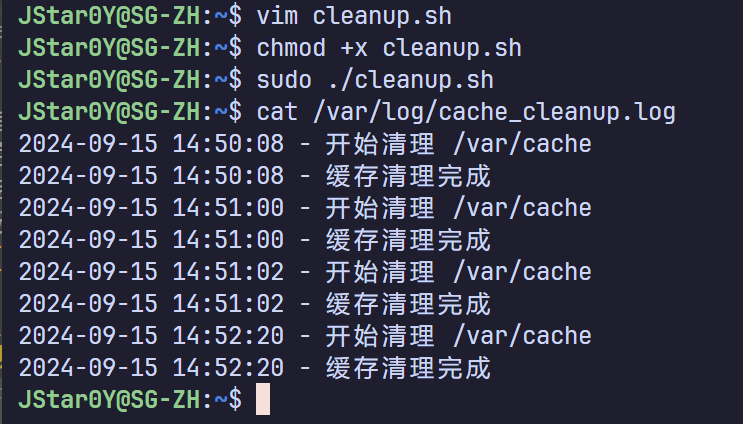
\includegraphics[width=0.8\textwidth]{Figures/cleanup_shell.png}
    \caption{Shell脚本实战:垃圾清理脚本执行结果}
    \label{fig:shellscript3}
\end{figure}

这种自动化缓存清理脚本也可以通过 \texttt{cron} 定时任务配置定期运行,可以有效简化系统运维工作量。